\documentclass[fleqn,10pt]{wlscirep}
\title{Automated Comment and Notebook Generation for Python Code}

\usepackage{graphicx}
\usepackage[export]{adjustbox}

\author[1,+]{Mayukh Nair}
\author[1,+]{Sanchit Bansal}
\author[1,+]{Vinayak Agarwal}
\author[1]{Anjali Goyal}
\author[1,*]{Ashish Sureka}

\affil[1]{Department of Computer Science, Ashoka University, India}

\affil[*]{Corresponding author: Ashish Sureka (ashish.sureka@ashoka.edu.in)}

\affil[+]{these authors contributed equally to this work}

%\keywords{Code Comments, Notebook Generator, Program Analysis, Abstract Syntax Trees}

\begin{abstract}
Documenting code is highly integral to ensuring that people reading the code can fully understand the processes taking place and extend the code properly, thus making it crucial for educational as well as archival purposes. A unique approach to documentation of code files, usually a manual and cumbersome task, has been proposed here by means of a series of programs which perform an analysis of written Python code and automatically generates comments for some logical operations of the code, as well as compiling a Jupyter / Interactive Python (IPython) Notebook from which formatted text and code can be exported to a variety for formats. This approach to documentation has a variety of applications which includes a simpler and elegant method to document code for amateur programmers and educators, as well as simplify creating Jupyter Notebooks from less feature rich development environments and text editors.

\end{abstract}
\begin{document}

\flushbottom
\maketitle
% * <mayukh.nair_ug18@ashoka.edu.in> 2018-05-03T19:42:31.197Z:
%
%  Click the title above to edit the author information and abstract
%
\thispagestyle{empty}

\section*{Introduction}

Software professionals agree that documentation of existing code is highly crucial to the development process, however this is impeded by the complexity of documentation tools which make it difficult to maintain code. A survey conducted by Forward et al. on tools and technologies for software documentation reported that developers preferred automated documentation tools, as well as the simplicity that word processors provide\cite{Forward:2002:RSD:585058.585065}. Most documentation tools require a great deal of manual work and learning which does not give the developer a self-motivated incentive to present their code in elegantly documented formats. 

Python is a programming language that is easy to learn and has a simple but effective approach to object-oriented programming\cite{van2003introduction}, and is widely preferred for multiple applications. There are multiple documentation tools available for code written in Python, such as Sphinx\cite{brandl2009sphinx}, however they suffer from the before-mentioned issue of being complicated and cumbersome to implement. Such tools deter first-time amateur programmers as well as educators from creating detailed documentation for the code they write. 

Python, like many other programming languages, offers in-built support for breaking down syntactically correct program code into an abstract tree representation of the same, known as an Abstract Syntax Tree (AST). AST allows programmatic access to the structure of written syntactic code and can be utilized to access underlying objects defined in code, their values and operations performed, which can be used to generate comments on values held and processes performed.

Jupyter\cite{kluyver2016jupyter} is a language-agnostic command shell that offers an interactive interface and an interface akin to a notebook which can be formatted, host images and other interactive content, and be presented in a variety of file formats in an elegant manner. Code can be viewed, run and modified live in Jupyter notebooks, thus making them an ideal tool for both code writing as well as documentation. 

A set of tools, written on the Python programming language and powered by libraries written for the language, allow the line-by-line analysis of code and automatically creates comments that can indicate the value or range that variables in code can inherit. A simplified commenting process to enter the author's text and notes which supports Markdown\cite{gruber2004markdown} for formatting plain text allows the code to be converted into Jupyter notebooks, which can then be exported to a variety of file formats. This is presented in an easy to use web interface which converts code in plain text into auto-commented and richly formatted code. 

\section*{Methods}

\subsection*{Approaches}

A primary goal for auto generation of code was to return the runtime values of the variables declared in the python code.
We tested several methods to solve the issue:

\begin{itemize}
\item \textbf{Memory} location of Variable : Aim was to use the function \textbf{id()} of python to obtain the memory address of each variable and access that memory after program execution.However there were several drawbacks to this approach. First, memory could have been allotted to something else once program execution was over. Second, we would not be able to track changes to the value of the variable.
\item \textbf{Abstract Syntax Tree} (AST) : The \textit{ast} module helps Python applications to process trees of the Python abstract syntax grammar. Previous work on ast had been used to visualize the program structure only. Parsing the python code to create a tree made it difficult to obtain flow of code based on tree traversal. External tracking of changes to variable values had to be implemented via dictionary. AST does not evaluates program expressions. Recursiveness of expressions - eg. x = x+(y/2) was tackled by using functions and recursive programming. Complex object referencing had to be implemented to traverse the tree.
\end{itemize}

\subsection*{Code structure}
The code is divided into four distinctive programs, built on the Python programming language, each of which perform a distinct task. All of these programs connect to each other sequentially to form as the part of a web application which does not require any user setup.
\begin{itemize}
\item \textbf{app.py}: This is the code that powers the graphical front-end for the web application, and uses the Flask and Django libraries for interactive web applications on a Python-powered back-end, and consists of Python code which controls a web interface written in HTML5, CSS and JavaScript. The interface offers a text field for the user to paste their written code in, and choose a format which they want their documented code in. 
\item \textbf{comment.py}: This code converts the Python code submitted through the front-end into an abstract syntax tree (AST), which is then parsed by traversing the nodes and accessing the values and attributes for each object and expression. A series of techniques to access the AST, as mentioned in the Approaches section, and tracking the initial and changed values of variables is used to generate a set of comments. This is output as a dictionary with the keys as the line on which a comment is autogenerated, and the comment itself as the value.
\item \textbf{autocomment.py}: The dictionary provided by comment.py is inserted into the original code here on a line-by-line basis.
\item \textbf{autodocgen.py}: The commented code is now analyzed line by line. Python-recognized comments (represented by a hash symbol at the start) which contain an asterisk at the beginning of the line are interpreted as plain text, and any Markdown formatting within it is parsed. Other lines are treated as lines of code, and additional code detects code blocks and formats them into cells, the basic unit of a Jupyter notebook. This is then used to generate a Jupyter notebook and export it to formats using the \textit{nbformat} and \textit{nbconvert} libraries. 
\end{itemize}

\begin{figure}[h!]
\centering
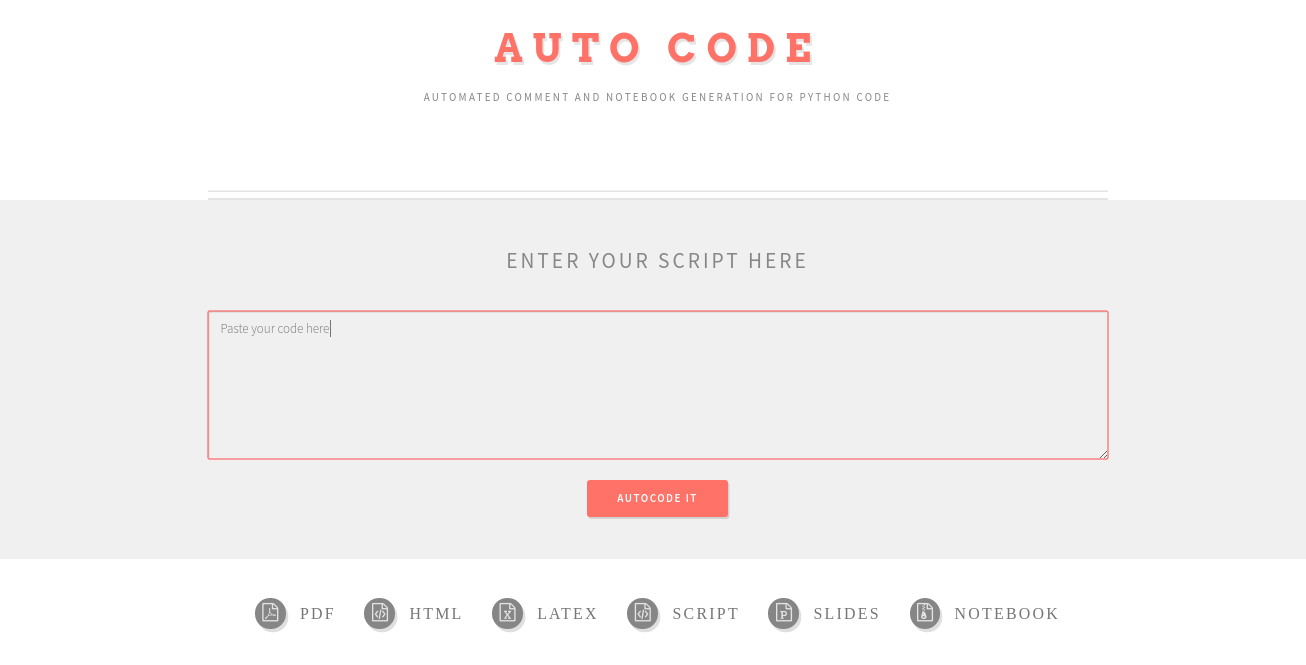
\includegraphics[width=\linewidth, frame]{screenshot}
\caption{Screenshot of the user interface, powered by \textit{app.py}.}
\label{fig:screenshot}
\end{figure}

\section*{Results}
The various programs are able to work in sequence and generate automatically commented and richly documented versions of the code input by the user. \textit{comments.py} generates a variety of comments which indicate variable declarations, as well as computed results of variable values and mathematical operations. A sample of the comments generated are as shown below.

\begin{verbatim}
x=8 # Value of variable x was 8
y= x**8 # Value of variable y was 16777216
x = y - (x**5) # Value of variable x was 16744448
print (y+(x%6)) # Value printed = 16777218
if x==y:
    print (x)
else:
    x=x+3 # Value of variable x was 16744451
\end{verbatim}

The commented code is then formatted to appear in a Jupyter notebook, and can be exported to one of six formats: PDF, HTML, \LaTeX, Script, Slides, or an .ipynb notebook.

\begin{figure}[h!]
\centering
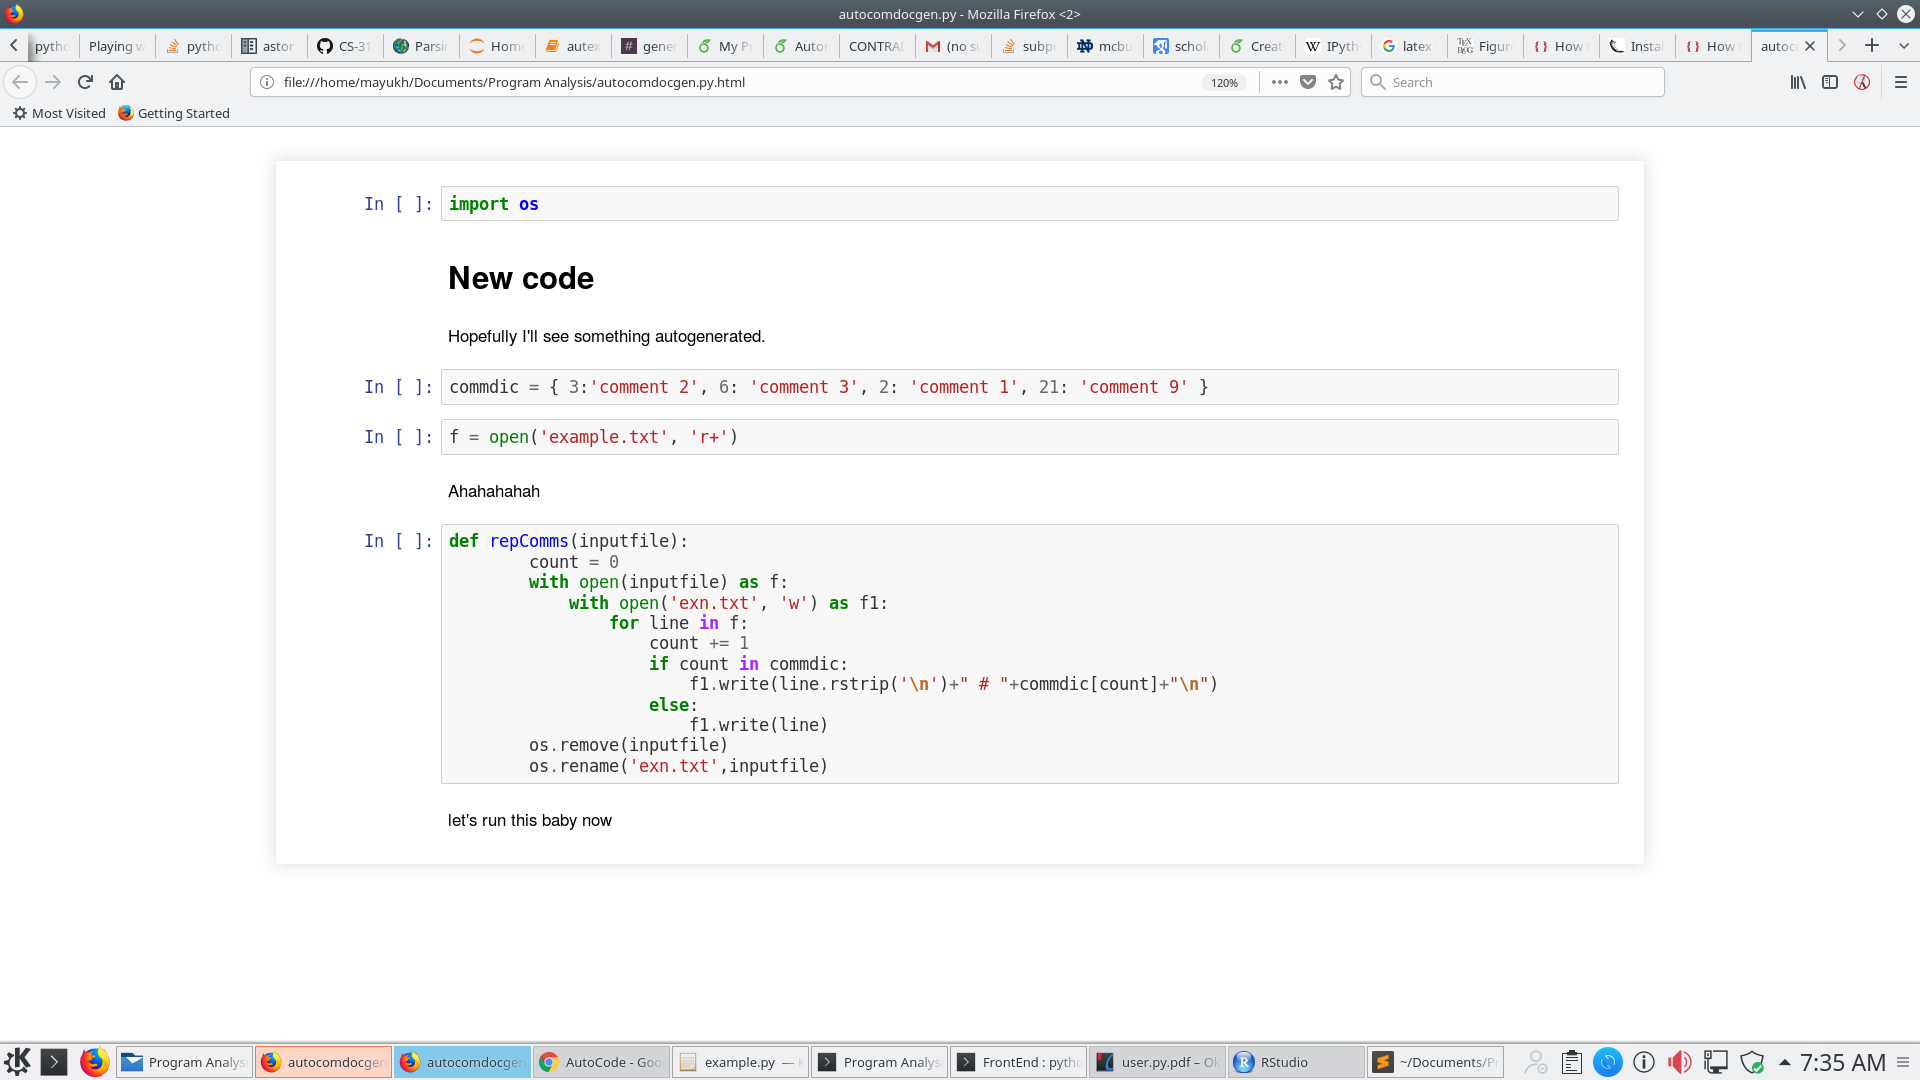
\includegraphics[width=\linewidth]{notebook}
\caption{Auto-generated HTML output of formatted and generated notebook.}
\label{fig:notebook}
\end{figure}

\bibliography{refs}

\section*{Author contributions statement}

M.N., S.B. and V.A conceived the project idea,  M.N. was responsible for \textit{autocomment.py} and \textit{autodocgen.py}, S.B. was responsible for app.py and the user interface and V.A. was responsible for comment.py and integrating the different programs into a sequential processing system. A.G. and A.S. supervised the project and offered feedback and guidance towards the same. M.N, S.B. and V.A. reviewed the manuscript.

\section*{Additional information}

The program is parsed to create a tree. Every node is hence traversed using a for loop. For every node, we check if its an assignment/expression/if-else statement.

\end{document}